\section{Closure test datasets}
\label{sec:appendix-datasets}

The full list of datasets included in the test set are shown in
Tab.~\ref{tab:summarise_new_data}. The central values are not actually used
in the closure test, however we use the experimental uncertainities in
the calculation of both $\biasvarratio$ and $\xisigdat{1}$. The corresponding
predictions generated from the underlying law are used as the true
observable values. Neither of the data-space closure estimators rely on
the central values of the test datasets.

\begin{table}[h!]
    \begin{center}
        \begin{tabular}{lc}
    \toprule
    Data set
    & Ref.
    \\
    \midrule
    DY E906 $\sigma^d_{\rm DY}/\sigma^p_{\rm DY}$ (SeaQuest)
    & \cite{Dove_2021}
    \\
    \midrule
    ATLAS $W,Z$ 7 TeV ($\mathcal{L}=4.6$~fb$^{-1}$)
    & \cite{Aaboud:2016btc}
    \\
    ATLAS DY 2D 8 TeV
    & \cite{Aaboud:2017ffb}
    \\
    ATLAS high-mass DY 2D 8 TeV
    & \cite{Aad:2016zzw}
    \\
    ATLAS $\sigma_{W,Z}$ 13 TeV
    & \cite{Aad:2016naf}
    \\
    ATLAS $W^+$+jet 8 TeV
    & \cite{Aaboud:2017soa}
    \\
    ATLAS $\sigma_{tt}^{\rm tot}$ 13 TeV ($\mathcal{L} = \SI{139}{\per\femto\barn}$)
    & \cite{Aad:2020tmz}
    \\
    ATLAS $t\bar{t}$ lepton+jets 8 TeV
    & \cite{Aad:2015mbv}
    \\
    ATLAS $t\bar{t}$ dilepton 8 TeV
    & \cite{Aaboud:2016iot}
    \\
    ATLAS single-inclusive jets 8 TeV, R=0.6
    & \cite{Aaboud:2017dvo}
    \\
    ATLAS dijets 7 TeV, R=0.6
    & \cite{Aad:2013tea}
    \\
    ATLAS direct photon production 13 TeV
    & \cite{Aaboud:2017cbm}
    \\
    ATLAS single top $R_{t}$ 7, 8, 13 TeV
    & \cite{Aad:2014fwa,Aaboud:2016ymp,Aaboud:2017pdi}
    \\
    \midrule
    CMS dijets 7 TeV
    & \cite{Chatrchyan:2012bja}
    \\
    CMS 3D dijets 8 TeV
    & \cite{Sirunyan:2017skj}
    \\
    CMS $\sigma_{tt}^{\rm tot}$ 5 TeV
    & \cite{Sirunyan:2017ule}
    \\
    CMS $t\bar{t}$ 2D dilepton 8 TeV
    & \cite{Sirunyan:2017azo}
    \\
    CMS $t\bar{t}$ lepton+jet 13 TeV
    & \cite{Sirunyan:2018wem}
    \\
    CMS $t\bar{t}$ dilepton 13 TeV
    & \cite{Sirunyan:2018ucr}
    \\
    CMS single top $\sigma_{t}+\sigma_{\bar{t}}$ 7 TeV
    & \cite{Chatrchyan:2012ep}
    \\
    CMS single top $R_{t}$ 8, 13 TeV
    & \cite{Khachatryan:2014iya,Sirunyan:2016cdg}
    \\
    \midrule
    LHCb $Z\to \mu\mu, ee$ 13 TeV
    & \cite{Aaij:2016mgv}
    \\
    \bottomrule
\end{tabular}
    \end{center}
    \caption{
        Observables included in the test data. We wish to stress that the observable
        central values themselves are not used, however the experimental
        uncertainities are used in the definition of the closure estimators, and
        the corresponding predictions from either the underlying law or the
        closure fits.
    }
    \label{tab:summarise_new_data}
\end{table}

For completeness, in Fig.~\ref{fig:DataKinematicCoverage}
the kinematic coverage of the training datasets, which
as mentioned is the NNPDF3.1-like dataset used in \cite{Faura_2020}, and the
test datasets shown in Tab.~\ref{tab:summarise_new_data} is plotted.

\begin{figure}
    \centering
    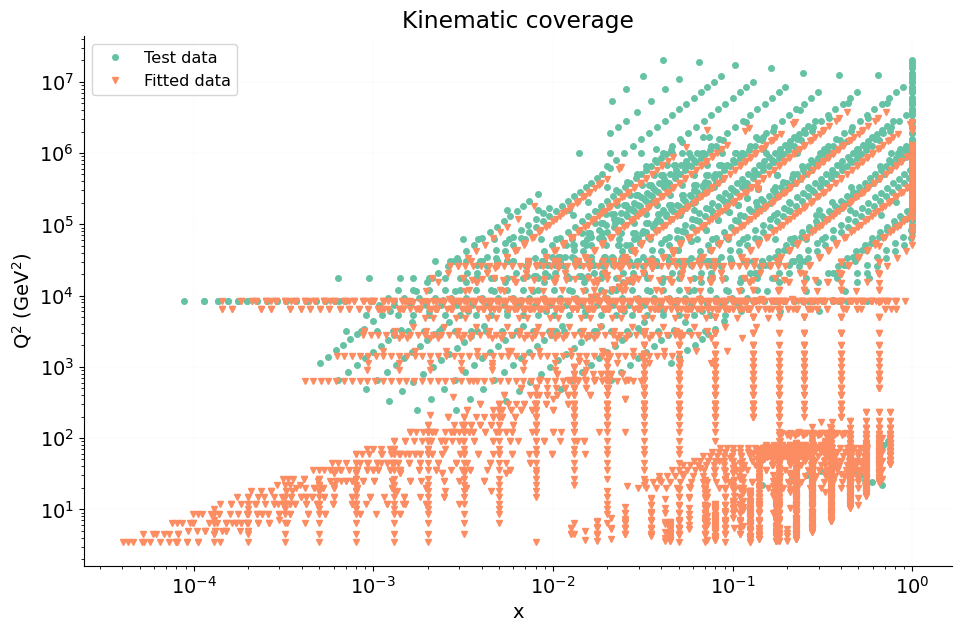
\includegraphics[width=0.8 \textwidth]{plot_xq2.png}
    % TODO: make PDF for higher res image.
    \caption{The kinematic coverage of the training and test data
    used to train the models and produce results presented in this paper. We emphasise
    that the split of datasets was largely chosen on practical grounds, not because
    of a deep reason to split the data chronologically. The kinematics of the two
    sets of data with this particular split overlaps but there are also kinematic
    regions which the test dataset probes, for which there was no training data.}
    \label{fig:DataKinematicCoverage}
\end{figure}
